% Section 4 draft. Numbers come from notebooks/notebook.ipynb (re-check them against the final run).
% FLAIRS rules: no \input (tables are inline), no caption/geometry/titlesec packages.
% Tables use plain \hline rules (no vertical lines), so no extra package is needed.
\section{Experiments}

\subsection{Datasets \& Exploratory Statistics}
We use three public datasets (Table~\ref{tab:data}). Panther telemetry and mortality records come from the Florida Fish and Wildlife Conservation Commission (FWC) \cite{FWCPantherTelemetry,FWCPantherMortality}; the road network is the Florida Department of Transportation (FDOT) Linear Referencing System (LRS) Routes with Measures layer \cite{FDOTLRS}. All layers are reprojected to a common metric coordinate system (North American Datum 1983 (NAD83), Universal Transverse Mercator (UTM) zone 17N, EPSG:26917) so that buffers, distances, and spatial blocks are measured in meters.

\begin{table}[t]
\centering
\small
\begin{tabular}{lrr}
\hline
\textbf{Dataset} & \textbf{Raw} & \textbf{In scope} \\
\hline
Telemetry fixes & 112{,}802 & 63{,}170 \\
Vehicular deaths & 461 & 399 \\
Road routes & 18{,}405 & 765 \\
\hline
\end{tabular}
\caption{Dataset sizes before and after scoping.}
\label{tab:data}
\end{table}

We keep telemetry fixes and vehicular-trauma deaths from 2000 onward, and roads and deaths in Collier, Hendry, Lee, and Glades counties, the study area defined in the Introduction. This leaves 63{,}170 fixes from 219 panthers, 399 vehicular deaths, and 765 road routes (3{,}838~km). Telemetry fixes were collected by aerial very high frequency (VHF) radio tracking, and 98.8\% of the 2000+ fixes were recorded between 07:00 and 17:00, so consecutive fixes are sparse snapshots rather than continuous tracks. We start in 2000 because recorded vehicular deaths rise sharply from that year onward, and this cutoff retains 93.5\% of all vehicular deaths (431 of 461) while discarding the sparsely recorded early years.

Routes are split at every intersection into $N=2{,}631$ road segments (median length 600~m), which are the nodes of the graph. The graph has 5{,}637 physical-adjacency edges and 243 movement-derived edges, 174 of which link segments that are not physically adjacent. A segment is labeled positive if a vehicular death lies within a buffer distance $b$ of it. At $b=100$~m, 163 segments (6.2\%) are positive; at 250~m and 500~m, 194 (7.4\%) and 218 (8.3\%) (Table~\ref{tab:labels}). Because positives are this rare, a trivial ``no strike'' predictor, which labels every one of the $N$ segments negative, would exceed 90\% accuracy at every buffer (the no-strike accuracy column of Table~\ref{tab:labels}), so we do not report accuracy.

\begin{table}[t]
\centering
\small
\begin{tabular}{rrrr}
\hline
\textbf{$b$ (m)} & \textbf{Positives} & \textbf{Positive rate} & \textbf{No-strike accuracy} \\
\hline
100 & 163 & 6.2\% & 93.8\% \\
250 & 194 & 7.4\% & 92.6\% \\
500 & 218 & 8.3\% & 91.7\% \\
\hline
\end{tabular}
\caption{Label imbalance by buffer distance $b$.}
\label{tab:labels}
\end{table}

\subsection{Baselines}
We compare against three baselines. \textbf{Random forest} \cite{Breiman2001} (300 trees, minimum leaf size 3, class-weighted) and \textbf{XGBoost} \cite{Chen2016XGBoost} (300 trees, depth 4, learning rate 0.05, positive-class weight set to the training class ratio) use the same 13 node features as the graph model (Table~\ref{tab:features}) but no graph structure; they are standard tree-based baselines for imbalanced tabular prediction, and random forests have been used for wildlife--vehicle collision risk \cite{pagany2022spatiotemporal}. A \textbf{kernel density} baseline fits a Gaussian kernel density estimate (KDE; bandwidth 2~km) to historical deaths in the training folds and scores each test segment at its midpoint, projecting past strikes onto the road network without using features. To isolate the contribution of movement connectivity, we also train an adjacency-only variant of the graph model that uses the physical-adjacency edges alone, on the same folds.

\begin{table*}[t]
\centering
\small
\begin{tabular}{ll}
\hline
\textbf{Feature} & \textbf{Definition} \\
\hline
Crossing frequency & Movement steps (fixes at most 30 days apart, joined by a straight line) crossing the segment \\
Fixes within 500~m and 2~km & Telemetry fixes within each distance of the segment \\
Panthers within 2~km & Distinct panthers with a fix within 2~km of the segment \\
Distance to nearest fix & Meters from the segment to the closest telemetry fix \\
Segment length & Length of the segment in meters \\
Road status & FDOT road status code, one indicator per code (7 codes) \\
Label & 1 if a vehicular death lies within $b$ of the segment, else 0 \\
\hline
\end{tabular}
\caption{Node features and label.}
\label{tab:features}
\end{table*}

\subsection{Evaluation Metrics}
Let $y_i\in\{0,1\}$ be the label of segment $i$ and $s_i$ a model's risk score. Metrics are computed on each held-out fold and reported as mean $\pm$ standard deviation.
\textbf{Area under the precision-recall curve (AUC-PR)}, the primary metric, is the average precision of the ranking by $s_i$; a random scorer scores about the positive rate (0.062 at $b=100$~m).
\textbf{Recall at the top $p$\%}, for $p\in\{5,10\}$, is the fraction of a fold's positive segments that appear among its $p$\% highest-scoring segments, reflecting the share of mortality an agency would capture by treating that fraction of the road network; a random scorer scores $p$\%.
\textbf{Brier score} $\frac{1}{N_f}\sum_i (s_i-y_i)^2$, averaged over the $N_f$ segments of a held-out fold, measures calibration when the risk score $s_i$ is a predicted probability (lower is better); it is undefined for the KDE baseline, whose output is a density.

\subsection{Evaluation Protocol}
Random $k$-fold splits would place neighboring, graph-connected segments in both training and test sets. We instead use spatial block cross-validation: segment midpoints are assigned to 15~km square blocks (67 blocks), and whole blocks are assigned to $5$ folds, largest first, to balance fold sizes (Figure~\ref{fig:folds}). Each fold holds about 526 segments; at $b=100$~m the number of positive segments per fold ranges from 18 to 41 (positive rate 3.4\% to 7.8\%), and the number of vehicular deaths from 33 to 145. Each model is trained on four folds and tested on the fifth; all models, including the graph model, use identical folds, and each death is assigned to the fold of its nearest segment so the KDE is fit only on training-fold deaths. Hyperparameters are fixed in advance and not tuned, so no separate validation split is needed; this avoids selecting settings on test folds. Paired per-fold differences are used to check that a model's advantage is consistent rather than driven by one fold.

\begin{figure}[t]
\centering
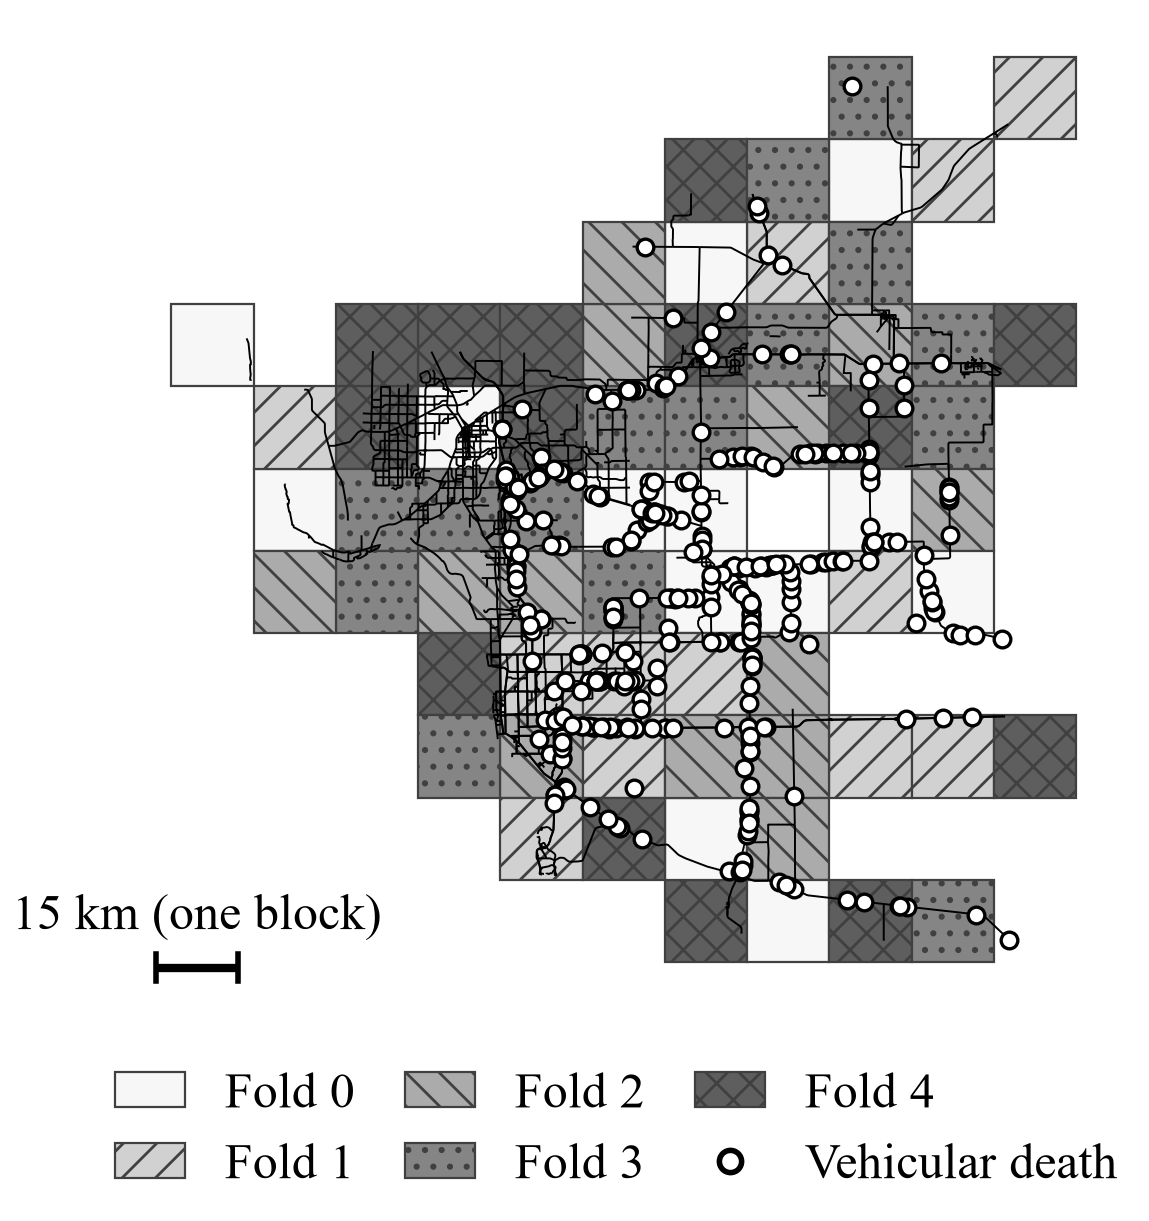
\includegraphics[width=\columnwidth]{figures/study_map_folds.png}
\alt{Map of the four-county study area. Road segments are drawn as black lines over 15 kilometer square blocks, each shaded and patterned by one of five cross-validation folds. Open circles mark vehicular deaths, which concentrate along a few major roads in the center and west.}
\caption{Road segments, vehicular deaths, and the five spatial cross-validation folds.}
\label{fig:folds}
\end{figure}

\subsection{Reproducibility}
All experiments are run from a single Jupyter notebook that reads the three datasets and fixes every parameter in one configuration cell: movement-step gap limit (30 days), minimum movement-edge weight (2), maximum segments per step (6), label buffers (100/250/500~m; 100~m for the main results), block size (15~km), and random seed (42). Software versions are Python with scikit-learn 1.9.0, XGBoost 3.4.1, GeoPandas 1.1.4, Shapely 2.1.2, and NetworkX 3.6.1. The notebook, datasets, and a dataset README are provided with the submission.
